%% 	This LaTeX Template is meant for "Second Bachelor´s Thesis"
%% 	written by Frank A Titze in March 2009
%% 	for Hochschule Kufstein Tirol, Austria, Dep. Wirtschaftsinformatik
%% 	www.hsk-edu.at
%% 	@author Frank A Titze (frank.a.titze@gmx.eu)
%% 	@copyright 2009, FAT
%% 	@license GPL
%% 	@version 1.0
%%=================================================
%% 	Main Document  Vorlage_BA2_by.fat.tex
%% 	This document:  mainmatter.tex
%%=================================================

%% Hier soll der Hauptteil der Arbeit erscheinen
%% auskommentieren der folgenden Zeile entfern den Beispielcontent
%% %% 	This LaTeX Template is meant for "Second Bachelor´s Thesis"
%% 	written by Frank A Titze in March 2009
%% 	for Hochschule Kufstein Tirol, Austria, Dep. Wirtschaftsinformatik
%% 	www.hsk-edu.at
%% 	@author Frank A Titze (frank.a.titze@gmx.eu)
%% 	@copyright 2009, FAT
%% 	@license GPL
%% 	@version 1.0
%%=================================================
%% 	Main Document  Vorlage_BA2_by.fat.tex
%% 	This document:  beispiele.tex
%%=================================================

%% Zusätzliche Trennvorschriften:
\hyphenation{op-tical net-works semi-conduc-tor e-com-merce Top-Ma-na-ge-ment}


\chapter{Beispielcontent}


\section{Quellenverweise}

Die Sache mit dem Zitieren ist eine Geschichte voller Missverständnisse. Zuerst gibt es da nämlich die Unterscheidung zwischen Kurz- und Langzitaten.

Ein sogenanntes Kurzzitat ist ein Verweis im Text, der auf Autorenname(n) und Jahreszahl besteht \cite[vgl.][S.72]{Jarz2008}. Es ist uns freigestellt, ob wir wie hier den Literaturverweis direkt in den Text einbauen wie in einschlägiger Literatur meist anzutreffen, oder -- wie es dem Herrn Jarz ganz gut gefällt -- über Fußnoten unsere Quellenangaben machen. Für die Sache mit den Fußnoten habe ich deshalb auch etwas eingebaut\footcite[S.39]{Jarz2008}. 

Ein Lang- oder Vollzitat hingegen ist eine komplette Quellenangabe, so wie wir es ins Quellenverzeichnis hinten im Dokument schreiben. So etwas stünde immer in einer Fußnote, ist meines Erachtens aber überflüssig, da wir ja ein Quellenverzeichnis haben. Daher sollten Verweise im Text ausreichen.\footcite{paula}

Um die Formatierung des Quellenverzeichnis übrigens müssen wir uns nicht weiter kümmern, solange alle relevanten Daten über JabRef in der Literaturdatenbank eingetragen sind, \BibTeX~ sei Dank.







\section*{Sectionüberschrift ohne Nummerierung}
Hier eine Sectionüberschrift ohne Nummerierung: Das geht auch mit anderen Überschriften, und liegt an dem angefügten Stern im Code.



\section{Liste mit Punkten}
\begin{itemize}
\item Punkt1 mit Text
\item Noch etwas
\item Und was ganz anderes
\item Ebenso ein Schmarrn
\end{itemize}



\section{Nummerierte Liste}
\begin{enumerate}
\item Punkt1 mit Text
\item Noch etwas
\item Und was ganz anderes
\item Ebenso ein Schmarrn
\end{enumerate}



\section{Liste Description}
\begin{description}
\item[davor] Punkt1 mit Text
\item[lalala] Noch etwas
\item[huhuu] Und was ganz anderes
\item[undso] Ebenso ein Schmarrn
\end{description}



\section{Ein Bildchen}
Ein Verweis auf ein Bild (wie z.B. Abbildung~\ref{fig:texlogo} auf Seite~\pageref{fig:texlogo} ) im geschriebenen Text wird immer per Nummerierung gemacht, nie mit einem Doppelpunkt nach einem Satz der vor dem Bild zu stehen hat. 

\begin{figure}[!t]
	\centering
			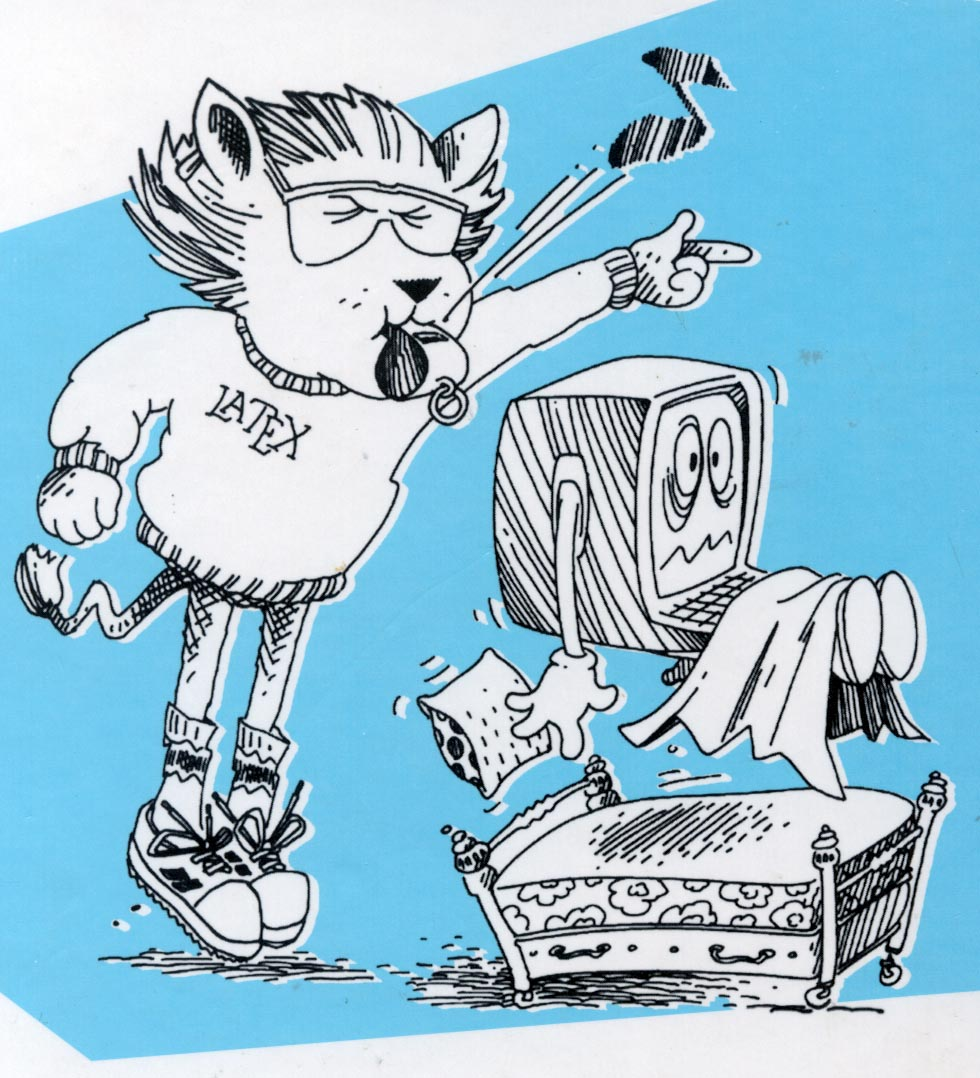
\includegraphics[width=0.5\textwidth]{misc/latex.jpg} 		% Bild relativ zur Textbreite skalieren
	   	  \caption[\LaTeX~Logo] % Dieser Text hier erscheint im Abbildungsverzeichnis
	   	  				{Und dieser Text hier erscheint schlussendlich direkt unterhalb des Bildes. Daher kann hier durchaus auch etwas mehr stehen.}
  			\label{fig:texlogo}
\end{figure}






\section{Textformatierungen}

In diesem Text werden ein paar wenige, aber übliche Formatierungen dargestellt,
je nachdem ob man \textbf{fett} drucken möchte, \textit{kursiv} oder \underline{unterstrichen}, aber auch die \emph{Hervorhebung}
gewisser Terme könnte von Vorteil sein.

Obacht! Fettdruck im normalen Fließtext sollte NIEMALS nötig sein\footcite[S.112]{Jarz2008}.

Gerade für Sourcecode bietet sich die \texttt{Schreibweise mit fester Laufweite} an. Für Namen würde sich eventuell auch
die Verwendung echter \textsc{Kapitälchen} anbieten, für welche ganz explizit \LaTeX~sehr bekannt ist.

Termini technici werden oft auch \textsl{slanted} oder \textit{kursiv} dargestellt, mit kleinen Unterschieden.

\section{Ein herausgestelltes Zitat}
\begin{zitat}
		"`Graecum te, Albuci, quam Romanum atque Sabinum,
		municipem Ponti, Tritani, centurionum,
		praeclarorum hominum ac primorum signiferumque,
		maluisti dici. Graece ergo praetor Athenis,
		id quod maluisti, te, cum ad me accedis, saluto:
		'chaere,' inquam, 'Tite!' lictores, turma omnis chorusque:
		'chaere, Tite!' hinc hostis mi Albucius, hinc inimicus."'
\end{zitat}





\section{Eine einfache Tabelle}

Tabellen werden in der table-Umgebung gesetzt, um auch als Tabellen erkannt zu werden (siehe Tabelle~\ref{tab:WerkCicero} auf Seite~\pageref{tab:WerkCicero}). Fügte man hier beispielsweise das Bild oder PDF einer Excel-Tabelle ein, würde es ebenso  als Tabelle geführt. 

\begin{table}[!t]
	\centering
	\begin{tabular}{cll}\hline\hline
	Jahr & Originaltitel & engl. Titel \\ \hline
	84 BC & De Inventione & About the composition of arguments \\
	55 BC & De Oratore & About oratory \\
	54 BC & De Partitionibus Oratoriae & About the subdivisions of oratory \\
	52 BC & De Optimo Genere Oratorum & About the Best Kind of Orators \\
	46 BC & Paradoxa Stoicorum & Stoic Paradoxes \\
	46 BC & Brutus & For Brutus \\
	46 BC & Orator ad M. Brutum & About the Orator, dedicated to Brutus \\
	45 BC & De Fato & On Fate \\
	44 BC & Topica & Topics of argumentation \\ \hline\hline
	\end{tabular}
	\caption[Dies ist der Kurztitel fürs Verzeichnis]{Und hier steht dann derjenige Text, welcher direkt unterhalb der Tabelle zu finden ist.}
	\label{tab:WerkCicero} 	% Textmarke
\end{table}






\section{Verweise und Referenzen}
\label{sec:references}
Indem man \verb+\label+ im Code vergibt, kann man mit \verb+\ref+ direkt darauf verweisen, und mit \verb+\pageref+ sogar die Seitennummer angeben. Als Rückgabewert kommt bei Bildern und Tabellen die jeweilige Nummerierung, bei Überschriften die Gliederungsnummer. An dieser Stelle verweise ich auf Überschrift~ \ref{sec:references}, welche auf Seite~ \pageref{sec:references} steht.

Die Tilde im Code bedeutet, dass an dieser Stelle ein fester Leerraum steht, der nicht getrennt werden darf.




\section{Sourcecode einfügen}
Sourcecode wird in der \verb+\listings+ Umgebung gesetzt, mit vielen Möglichkeiten der Formatierung. Es wird fast jede Programmiersprache explizit unterstützt. Näheres unter \url{http://www.pvv.ntnu.no/~berland/latex/docs/listings.pdf}


\begin{lstlisting}[caption=Dies ist ein PHP Beispiel]{Beispiel}
public function delete(){
  if($_SESSION["loginstat"] == "v33PL")
  {
   $this->db_delete("bbericht", "IDbbericht", $_GET["id"], "");
  }else{
   $this->sec_msg();
  }
}
\end{lstlisting} 	%$ (Dieses Dollarzeichen ist nur eingefügt, da der Editor sonst denkt man hätte hier noch eine mathematische Formel-Umgebung offen, die zwischen Dollarzeichen gesetzt würde)




\section{Silbentrennung}

Sollte \LaTeX~wirklich einmal Probleme mit der Silbentrennung eines unbekannten Wortes haben, kann man über hyphenation
die Trennweise bekannt machen, oder auch das Trennen von Wörtern verbieten.
\begin{verbatim}
\hyphenation{er-go-no-mic} 		
\hyphenation{fortran}
\end{verbatim}
 "`fortran"' darf nie getrennt werden, "`ergonomic"' an den angegebenen Stellen






\section{Mathematische Formeln}
\LaTeX~ ist berühmt für seine einzigartigen Fähigkeiten im Umgang mit mathematischen Formeln.

Dabei gibt es die einfache Variante kurze Formeln wie $1+1=3$ direkt in den Text einzufügen, oder auch komplexere Formeln herausgehoben darzustellen, die dann auch nummeriert werden:

\begin{equation}%Beginn der Formel
t-t_{0}=\sqrt{\frac{l}{g}}\int_{0}^{\varphi}{\frac{d\psi}{\sqrt{1-k^{2}\sin^{2} {\psi}}}} = \sqrt{\frac{l}{g}} F(k,\varphi)
\end{equation}%Ende der Formel

\begin{equation}%Beginn der Formel
u(x,t)= 8 \frac{k_{1}^{2}e^{\alpha_{1}} + k_{2}^{2}e^{\alpha_{2}} + (k_{1}-k_{2})^{2}e^{(\alpha_{1}+ \alpha_{2})} \left[2 + \frac{1}{(k_{1} + k_{2})^{2}} ( k_{1}^{2}e^{\alpha_{1}} + k_{2}^{2}e^{\alpha_{2}}) \right]}{\left[1+e^{\alpha_{1}} + e^{\alpha_{2}} + \left(\frac{k_{1} - k_{2}}{k_{1}+k_{2}} \right)^{2} e^{\alpha_{1}+ \alpha_{2}} \right]^{2}}
\end{equation}%Ende der Formel






\section{Anführungszeichen}
Ein Satz mit "`Anführungszeichen"'.
Ein Satz mit französischen \frqq Anführungszeichen\flqq.
Ein Satz mit \textit{halben} französischen \frq Anführungszeichen\flq.



\section{Umlaute}
Sollten mal Probleme mit Umlauten auftreten, kann man sich mit den nativen Umlautzuweisungen behelfen:
\"a, \"A, \"o, \"O, \"u, \"U



\section{Abkürzungen}
Werden im Text Abkürzungen wie \gls{ad} für Active Directory benutzt, müssen diese vorher in der glossary-Datei definiert werden.
Von den zuvor definierten Abkürzungen werden aber nur diejenigen wirklich im Verzeichnis aufgeführt, welche auch im Texr verwendet wurden.
\gls{ad} wurde bereits verwendet mit \verb+\gls{ad}+. Ebenso \gls{ms}, aber CD wurde hier nicht als Code eingefügt, und fehlt daher im Verzeichnis.

Das besondere dabei: Bei der ersten Verwendung im Text wird die Abkürzung automatisch ausgeschrieben! Auch wird das Verzeichnis automatisch alphabetisch sortiert.




\section{Gliederungsebenen}
Die oberste Ebene ist das chapter, hier befinden wir uns gerade in einer section.
\subsection{Subsection}
\subsubsection{Subsubsection}
Spätestens hier sollte man mit Nummerierung aufhören!
\paragraph{Paragraph}
Und wer hier noch Nummerierung will, ist krank ;-)
\subparagraph{Subparagraph}




\section{Blindtext mit \LaTeX}
\lipsum





%%EOF@fat



 	% Einbinden der Beispiele


\chapter{Einleitung}
\label{ch:Einleitung}
Dieses Kapitel gibt eine Einführung in das Thema der Bachelorarbeit. Dabei wird auf die Ausgangssituation und den Aufbau der Arbeit eingegangen. Des weiteren wird die Problemstellung der Arbeit definiert und die Relevanz des Themas beschrieben.


\section{Ausgangssituation}

Anfangs war das Internet lediglich eine Informationsquelle für den Menschen. Mitte der 2000er-Jahre trat eine Veränderung ein, Internetnutzer wollten Teil des Webs werden, sie wollten selbst Inhalte generieren und mit anderen Internetnutzern teilen. So entwickelte sich das Internet zu einem interaktiven Web, welches unter dem Begriff des \dq Web 2.0\dq  durch Tim O'Reilly wesentlich geprägt wurde ZITIEREN \cite{oreilly}.

Auch hat die Zahl der Mobiltelefone in den letzten 15 Jahren sehr stark zugenommen.
Heutzutage sind Mobiltelefone und Internetzugang aus unserem alltäglichen Leben nicht mehr wegzudenken. Aus dem Mobile Communications Report 2017 der Mobile Marketing Assosiation Austria und der MindTake Research geht hervor, dass 2017 bereits 94\% der Österreicher ein Smartphone besitzen. 93\% der Österreicher nutzen das Internet regelmäßig auf ihrem Smartphone, in der Altersklasse der 15- bis 29-Jährigen, sind es sogar 100\%. Die tägliche Nutzung liegt bei über drei Stunden pro Tag. $[zitieren MMAA]$.

Die schnell voranschreitende Entwicklung neuer Technologien bietet Menschen sehr viele Möglichkeiten zu kommunizieren und sich mit anderen Menschen auszutauschen. Auch sind Menschen nicht mehr an das Internet zu Hause gebunden, sie können mobiles Internet auf ihren Mobiltelefonen, Tablets und Wearables unterwegs nutzen und live Informationen einholen. Die Entgeräte sind leistungsfähiger, benutzerfreundlicher, transportabel und intelligenter als je zuvor.

Bergsportlern stehen zahlreichen mobile Applikationen, Internetforen, Plattformen und Blogs für die Tourenplanung zur Verfügung. Touren können online angeschaut und geplant werden. Auf Interessensplattformen und Blogs beschreiben Bergsportler ihre eigenen Touren und berichten über ihre  Erlebnisse. Sie schreiben persönliche Reiseberichte mit vielen Details, diese können von anderen Internetnutzern gelesen und kommentiert werden. Eine Interaktion zwischen Verfasser, Leser und anderen Lesern entsteht. Diese Berichte können Bergsportlern als Motivation und Inspiration für zukünftige Touren dienen. Hier kann jedoch das Problem lauern, denn nicht jeder Bergsportler ist gleich fit und gleich erfahren.


\section{Problemstellung}

Das Angebot für Tourenplanung ist sehr groß, es reicht von gedruckten Tourenführern über Online-Plattformen zu GPS-fähigen Wearables. Bergtouren können heutzutage besser den je geplant werden, Online-Tools und mobile Applikationen geben Auskunft über die Distanz, Höhenmeter, Beschaffenheit der Strecke und Einkehrmöglichkeiten. Auch das Wetter ist jederzeit zeitnah abrufbar. Dennoch lässt sich der Presseaussendung von Januar 2018 des österreichischen Kuratoriums für alpine Sicherheit entnehmen, dass die Zahl der unverletzten Bergsportler, welche einen alpinen Notruf absetzen, in den vergangenen 10 Jahren stetig anstieg. Im Jahr 2017 machten Unverletzte bereits 37\% aller Notrufe aus. Alpine Notrufe werden nicht ausschließlich von tatsächlich Verunfallten und Verletzten abgesetzt, sondern auch von unverletzten Personen, die sich in einer misslichen Lage befinden ZITIEREN KURASI.
Um im weiteren Verlauf bessere Aussagen treffen zu können, widmet sich diese Arbeit den Wanderern. Wandern ist der beliebteste Bergsport und wird von Personen jeden Alters und Geschlechts ausgeübt.
In der Statistik der letzten 10 Jahre kann man entnehmen, dass die Zahl der Unverletzten von 425 im Zeitraum 01.11.2007 bis 31.10.2008 auf 811 im Zeitraum 01.11.2015 bis 31.10.2016 sich fast verdoppelte KLAMMER siehe Abbildung 1 KLAMMER. Die häufigsten Ursachen für einen Notruf von Unverletzten Personen sind \dq Verirren und Versteigen\dq gefolgt von \dq Erschöpfung\dq und \dq Wettersturz\dq. Es gibt durchaus Faktoren, die nicht vorhersehbar sind, dazu gehören Wettersturz, Blitzschlag, Steinschlag oder Herz-Kreislaufstörungen. Viele Faktoren können jedoch mit richtiger Vorbereitung und Planung durchaus minimiert werden. Recht hohe Zahlen KLAMMER zwischen 41 und 105 KLAMMER findet man unter dem Kriterium \dq Sonstiges\dq. Das bedeutet, dass keines der angegebenen Kriterien für das Absetzen eines Notrufes des Unverletzten zutraf. Hier stellt sich die Frage, ob es sein kann, dass der technische Fortschritt und die Menge an konsumierten Online-Inhalten dazu führt, dass sich Wanderer nach der Planungsphase und während der Ausübung der Sportart zu sehr in Sicherheit wiegen und eher für zu schwierige Touren entscheiden?

\section{Zielsetzung und Forschungsfrage}


Das Ziel der Bachelorarbeit ist es zu erforschen, wie weit  Wanderer von neuen Technologien und konsumierten Online-Inhalten bei der Risikobewertung einer Bergtour beeinflusst werden. Dabei soll einerseits untersucht werden, wie gut Wanderer, die ihnen zur Verfügung stehenden Technologien anwenden. Andererseits wird erforscht, wie Wanderer mit Online-Inhalten umgehen und die nützlichen Informationen filtern und mit ihren Fähigkeiten abgleichen. In einer qualitativen Umfrage soll herausgefunden werden, welche Technologien und Online-Inhalte Wanderer bevorzugt nutzen, um sich ein Bild von einer Tour zu machen. Des Weiteren soll herausgefunden werden, welchen Online-Inhalten Wanderer vertrauen und welche Inhalte für die Entscheidungsfindung, welche Tour tatsächlich gegangen wird, herangezogen werden.\\
Daraus lässt sich folgende Forschungsfrage ableiten: 
\textit{Wie werden Wanderer von Online-Inhalten und neuen Technologien bei der Risikobewertung einer Tour beeinflusst?}

\section{Aufbau der Arbeit}

Die vorliegende Bachelorarbeit \textit{Analyse des Entscheidungsverhaltens von Bergsportlern bei der Risikobewertung bei der Auswahl der Route beim Ausüben von Bergsport mit Zuhilfenahme von mobilen Applikationen und Online-Inhalten} besteht aus \# \# \# \# \# \# \# \# Kapiteln.\par

Im ersten Kapitel soll an das Thema der Arbeit herangeführt werden, die Relevanz und Problemstellung werden erläutert und eine Zielsetzung inklusive der Forschungsfrage werden dargestellt.\par

Die Kapitel \# \# \# \# \# \# \# \# enthalten die theoretischen Grundlagen.\par

Im \# \# \# \# \# \# \# \# Kapitel wird die Forschungsmethodik erläutert\par

Im \# \# \# \# \# \# \# \# Kapitel werden die Ergebnisse vorgestellt und die Arbeit schließt mit einem Fazit und Ausblick im \# \# \# \# \# \# \# \# Kapitel ab.

\chapter{Grundlagen}
\label{ch:Grundlagen}

Im folgenden Kapitel werden die grundlegenden Begriffe, welche für die Bachelorarbeit relevant sind, erläutert. 

\section{Web 2.0}
\label{web2.0}

Das Internet wurde in seinen Anfängen für Informations- und Darstellungszwecke benutzt. Dieses Konzept wird als Web 1.0 bezeichnet. Im Web 1.0 gibt es nur wenige Content-Ersteller, die überwiegende Mehrheit der Internetnutzer agiert lediglich als Konsument von Inhalten ZITIEREN KEY DIFFERENCES BETWEEN WEB1 u WEB2. Darauf folgte Anfang der 2000er Jahre das Konzept des Web 2.0. Der Begriff wurde von O'Reilly geprägt, wobei der Begriff bereits zuvor in Gebrauch war. Web 2.0 beschreibt keine neue Technologie sondern vielmehr eine veränderte Nutzung des Internets. O'Reilly beschrieb das Web 2.0 als eine Reihe von Prinzipien und Praktiken, die wie ein Sonnensystem von Websites miteinander verbunden sind, wobei einige oder alle dieser Prinzipien in unterschiedlichem Abstand vom Kern sind VGL O'REILLY ZITIEREN. O'Reilly sieht das Web 2.0 als eine von allen nutzbare Plattform mit Fokus auf datenbasierte Dienste.
Die Trennung, ob eine Internetseite eine Web 1.0 oder Web 2.0-Seite ist, lässt sich nur bei der Analyse mehrerer Achsen sichtbar machen. Dazu muss man sich die technische, strukturelle und soziologische Achse anschauen. Bei der technischen Achse betrachtet man die Präsentationstechnologie, die sowohl zur Darstellung der Webseite als auch zur Interaktion mit dem Benutzer verwendet wird. An der strukturellen Achse wird der Zweck und das Layout der Seite betrachtet und auf der soziologischen Achse werden die Freunde und Gruppen betrachtet VGL DIFFERENZES BETWEEN. \\
Durch die neu entstandene kollaborative Zusammenarbeit ist es möglich, das Wissen vieler Internetnutzer der Allgemeinheit zugänglich zu machen. Somit haben sich Webseiten im Web 2.0 so verändert, dass sie für die interaktive und kollaborative Nutzung die geeigneten Plattformen zur Verfügung stellen und die Webseiten laufend durch die Nutzerbeteiligung auf dem Aktuellen Stand gehalten werden. Durch die Nutzerbeteiligung wurden Webseiten und deren Inhalte dynamischer und flexibler.
Durch neue Technologien und das Verlangen des Internetnutzers, seine Erfahrungen, Kenntnisse und Gedanken mitzuteilen, entstand eine neue Interaktivität.



\section{Social Media}
\label{sozialMedia}

Während das Internet genutzt wurde, um die soziale Interaktion zu erleichtern, ermöglichte die Entstehung und schnelle Verbreitung von Web 2.0-Funktionalitäten im ersten Jahrzehnt des 21. Jahrhunderts einen Evolutionssprung in der sozialen Komponente der Webnutzung\footcite[S. 745-750]{obarSocialMedia} .\\
Für den Begriff Social Media gibt es viele Definitionen. Andreas M. Kaplan und Michael Haenlein beschreiben den Begriff Social Media als eine Gruppe von Internet-basierten Anwendungen, die auf den ideolotischen und technologischen Grundlagen des Web 2.0 aufbauen und die Erstellung und den Austausch von User Generated Content ermöglichen\footcite[S. 59-68]{kaplan}.\\
Kietzmann et al. verwenden eine Social Media Bienenwabe mit sieben funktionalen Bausteinen, welche die verschiedenen Ebenen von Social Media abbilden\footcite[S.241-251]{kietzmann}:

\begin{itemize}
	\item \textbf{Identität:} Offenbarung der Identität des Nutzers. Nach Kaplan und Haenlein ist die Identität eines Nutzer oft durch die bewusste oder unbewusste Selbstdarstellung subjektiver Informationen wie Gedanken, Gefühle, Vorlieben und Abneigungen gekoppelt\footcite[S.59-68]{kaplan}.
	
	\item \textbf{Gespräche:} dienen dem Nutzer um mit anderen Nutzern in einem Social Media Umfeld zu kommunizieren um beispielsweise Gleichgesinnte zu finden oder ihre Botschaft zu Gehör zu bringen.
	
	\item \textbf{Teilen:} Benutzer ändern, verteilen und empfangen Inhalte, darunter fallen z.B.: Text, Bild, Video, Ton, Link und Ort. Das Teilen ermöglicht Benutzern persönliche Objekte - Erfahrungen und Beobachtungen - mit der Welt zu teilen.
	
	
	\item \textbf{Präsenz:} Benutzer sehen, ob andere Benutzer erreichbar sind, dies soll eine Brücke zwischen der realen und der virtuellen Welt darstellen.
	
	
	\item \textbf{Beziehungen}
	
	
	\item \textbf{Reputation}
	
	
	\item \textbf{Gruppen}
\end{itemize}
















\section{Angewandte Modelle}
\label{ch:Modelle}

In diesem Teil wird auf die beiden gängigsten Modelle, dass Technology Acceptance Model von Fred D. Davis 

\subsection{Technology Acceptance Model}
\label{TAM}

Der wesentliche Faktor dieses Modells ist die Technikakzptanz \footcite[S. 319]{Davis}

\subsection{Task -Technology-Fit-Model}
\label{ch:TTF}

\cite{kurasi}

\cite{obarSocialMedia}
%%EOF@fat




